本章では提案手法の実装について述べる. 図 \ref{サーバ上の実装の概要} に実装の概要を示す. 提案手法はサーバクラスタによる分散グラフ処理システムであるため, 各サーバ上でこの実装によるプログラムが動作する. RWer 生成 \& 処理スレッドでは, RWer を生成しその後 RW 処理を行う. このとき他のサーバが所有する頂点への遷移が発生した場合は, その RWer を送信キューに格納する. 受信スレッドでは, 他のサーバからメッセージを受信し, そのメッセージの種類に応じた処理を行う. 例えばメッセージが複数の RWer を含むものだった場合は, それらの RWer を RWer キューに格納する. RWer 処理スレッドでは, RWer キューから RWer をまとめて取り出し, RW 処理を行い, 他のサーバが所有する頂点への遷移が発生した場合は, その RWer を送信キューに格納する. 送信スレッドでは, 送信先ごとの送信キューから RWer をまとめて取り出し, 他のサーバへ送信する. 以降, 終了した Random Walker の経路情報の保持方法, 受信スレッド, RWer 処理スレッド, 送信スレッドの 4 つについて, 適宜擬似コードを用いて詳細を説明する. 

\begin{figure}[t]
    \centering
    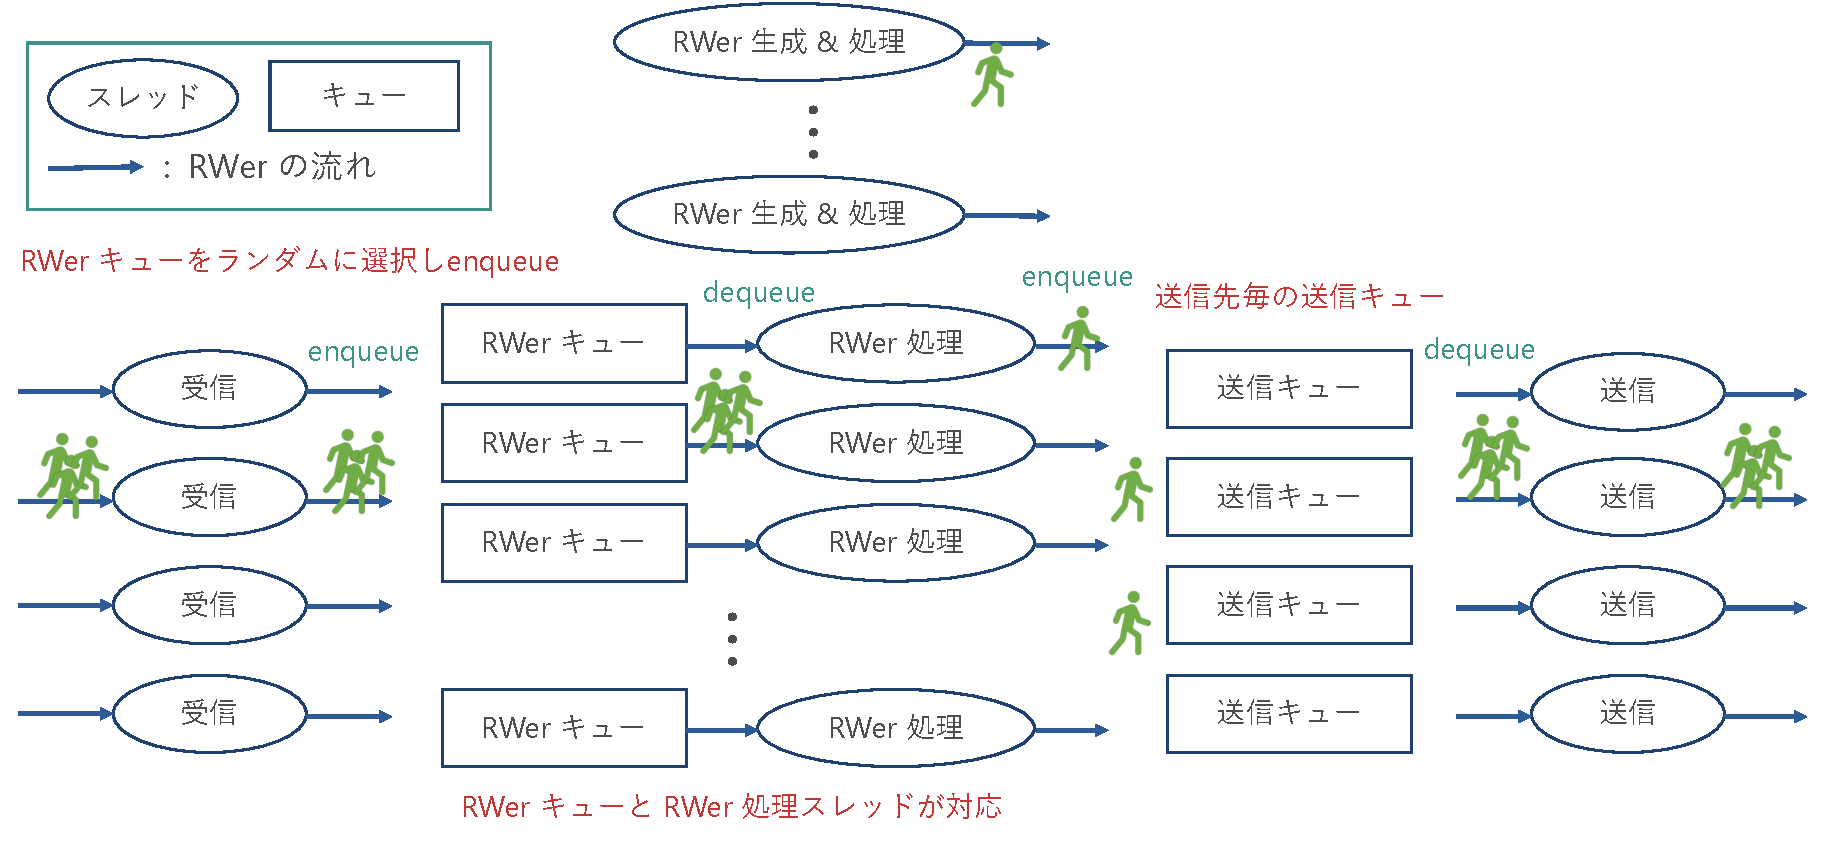
\includegraphics[scale=0.5]{figure/implementation.pdf}
    \caption{サーバ上の実装の概要.}
    \label{サーバ上の実装の概要}
\end{figure}

\section{終了した Random Walker の経路情報の保持方法}

\ref{Random Walker の経路再利用} で説明したように, 本手法では終了した RWer の経路情報を再利用することで通信のスキップを行う. そのためには終了した RWer の経路情報を保存しておく必要がある. 経路情報のまま保存するのは無駄が多いため, 経路再利用時に必要となる項目ごとに情報を保存する. 表 \ref{Random Walker の経路情報の保存形式} に RWer の経路情報の保存形式を示す. 本手法は C++ を使って実装しているためデータ構造は C++ の形式で記述した. 頂点に対する次数は RW 遷移時における index 選択の際に必要となる. データ構造に関しては, 頂点 ID を index とした配列の形で保持する. 頂点に対する持ち主サーバは, もし次の遷移先情報を持っていない場合に現在頂点の持ち主サーバへの RWer の送信が発生するため, 必要である. データ構造に関しては次数情報と同様, 頂点 ID を index とした配列の形で保持する. エッジデータは index を使った RW 遷移に必要となる. 例えば図 \ref{経路再利用による送信スキップ} ではサーバ 1 が (10, 0, 4), (10, 3, 11) (始点頂点, index, 遷移先頂点) というエッジデータを保持しているため, index = 0, 3 の場合は通信をスキップすることができる. データ構造に関しては, 頂点 ID を index とし, それぞれの頂点について (key, value) = (index, 遷移先頂点) のハッシュ map を保持する形とした. 

\begin{table}[t]
    \caption{Random Walker の経路情報の保存形式.}
    \label{Random Walker の経路情報の保存形式}
    \centering
    \begin{tabular}{cc}
        \hline
        保存項目  &  データ構造 (C++)  \\
        \hline \hline
        頂点に対する次数  &  std::vector$\langle$uint64$\_$t$\rangle$ \\
        \hline
        頂点に対する持ち主サーバ  &  std::vector$\langle$uint64$\_$t$\rangle$  \\
        \hline
        エッジデータ  &  std::vector$\langle$std::unordered$\_$map$\langle$uint64$\_$t, uint64$\_$t$\rangle$$\rangle$ \\
        \hline
    \end{tabular}
\end{table}

\section{受信スレッド}

\begin{algorithm}[t]
\DontPrintSemicolon
\nl $message \leftarrow$ 受信データ\;
\nl $message\_id \leftarrow message$ の先頭から抜き出した値\;
\nl \If{$message\_id ==$ 複数の RWer によるメッセージ} {
\nl     $RWer\_count \leftarrow message$ の先頭から抜き出した値\;
\nl     $RWer \;\; A[RWer\_count]$\;
\nl     $idx \leftarrow message$ 内における先頭の RWer 情報の開始位置\;
\nl     \For{$i = 1$ to $RWer\_count$} {
\nl         $A[i] \leftarrow message 内における i$ 個目の RWer の情報\;
\nl         $idx \leftarrow idx$ + ($i$ 個目の RWer のメモリサイズ)\;}
\nl     RWer キューをランダムに選択し, $A$ 内の RWer を全て格納\;}
\nl \Else{
\nl     他の場合は説明省略\;}
\caption{{受信スレッド} \label{受信スレッド}}
\end{algorithm}

\begin{table}[t!]
    \caption{メッセージの構成.}
    \label{メッセージの構成}
    \centering
    \begin{tabular}{ccc}
        \hline
        名称  &  サイズ  &  内容 \\
        \hline \hline
        $ver\_id\_$  &  8 bit  &  バージョン: 4 bit, メッセージ ID: 4 bit \\
        \hline
        $RWer\_count$  &  16 bit  &  メッセージ内に含まれる RWer の数 \\
        \hline
        複数の RWer  &  可変長サイズ $\times$ $RWer\_count$  &  表 \ref{RWer の構成} の RWer の情報を複数格納 \\
        \hline
    \end{tabular}
\end{table}

受信スレッドでは, 他のサーバから受信したメッセージを処理し, 適宜 RWer を RWer キューに格納する. メッセージの種類は複数の RWer 以外にも実験開始の合図, 結果送信の合図等があるが, ここでは主要な処理である複数の RWer について説明する. Algorithm \ref{受信スレッド} に受信スレッドの擬似コードを示す. また, 提案手法におけるメッセージ構成を表 \ref{メッセージの構成} に示す. まず, 受信したメッセージを $message$ に格納し, $message\_id$ を先頭の $ver\_id\_$ から抽出する (1, 2 行目). 次に $message$ からメッセージ内の RWer の個数である $RWer\_count$ を抽出し, サイズ $RWer\_count$ の RWer 格納用配列を作成する (4, 5 行目). そしてその配列 $A$ に $message$ 内の RWer の情報を格納していく(6 -- 9 行目). $idx$ は $message$ 内におけるそれぞれの RWer の情報の開始位置を表す. つまり, 6 行目において $idx$ = 24 bit であり, RWer の情報の開始位置は先頭から 25 bit 目である. RWer の情報は可変長なので, 2 つ目以降の RWer に関する $idx$ については, その都度一つ前の RWer のメモリサイズを表 \ref{RWer の構成} の $RWer\_size$ から読み取り, 加算する(9 行目). 最後に, 格納先の RWer キューをランダムに一つ選択し, $A$ 内の RWer を全て格納する(10 行目). 本手法では, 並列性を可能な限り保つことができる構築を意識しており, 受信スレッドごとに異なるポート番号を振り分け, 受信処理を並列に行う. また, RWer 処理スレッドも同様で, 図 \ref{サーバ上の実装の概要} のように各 RWer スレッドごとに RWer キューを用意した. 10 行目における RWer キューのランダム選択は, 各 RWer 処理スレッドの負荷分散のためである. また, $A$ 内の RWer それぞれに対してランダムな RWer キューを選択するのではなく, $A$ 内の全ての RWer をまとめて一つの RWer キューに格納するのは, RWer キューにて必要となる排他制御のロックを低減させるためである. 

本手法ではスレッド間での情報のやり取りが多い. 例えば, 受信スレッドと RWer 処理スレッド間では RWer キューを通じて RWer を受け渡す. ここでもし RWer を構造体のまま RWer キューへ push, または RWer キューから pull しようとすると, その都度構造体のメモリコピーが発生してしまいオーバヘッドが大きくなる. そのため本手法では情報の受け渡しをポインタで行う. また, スレッド間でのポインタの受け渡しには所有権の概念が存在するため, C++ におけるスマートポインタを利用してこの処理を実装した. 



\section{RWer 処理スレッド}

RWer 処理スレッドでは, RWer キューから RWer をまとめて取り出し, それぞれの RWer に対して RW 処理を行い, 他のサーバが所有する頂点への遷移が発生した場合は, その RWer を送信キューに格納する. Algorithm \ref{RWer 処理スレッド} に RWer 処理スレッドの擬似コードを示す. まず RWer キューから RWer をまとめて取り出し, 配列 $A$ に格納する(1, 2 行目). そして $A$ 内の各 $RWer$ について RW 処理を行う(3 -- 38 行目). RW 処理については, まず $RWer$ の $ver\_id\_$ (表 \ref{RWer の構成} 参照) から $message\_id$ を抽出し, それがもし終了した RWer のものだった場合, 終了した RWer に対する処理を行う(4 -- 6 行目). 終了した RWer に対する処理では主にその RWer の生成サーバに対応する送信キューへの push を行う. $message\_id$ が, まだ生存している RWer のものであった場合は, その RWer が終了 or 他のサーバが所有する頂点へ遷移し, 送信キューに格納されるまで処理を繰り返し行う(7 -- 38 行目). ここでの処理は $RWer$ の現在頂点である $current\_node$ (9 行目)が自サーバの所有頂点である場合とそうでない場合で異なる. $current\_node$ が自サーバの所有頂点である場合は, 基本的にはそのサーバが所持するグラフ上でのランダム遷移を行う. しかし 1 hop 前で通信が発生した, かつ $RWer$ の $next\_index\_$ (表 \ref{RWer の構成} 参照) に index 情報が格納されている場合は, 次の遷移はその index 情報を利用して行う(11 -- 14 行目). これは図 \ref{経路再利用による送信スキップ} の送信が発生したときのサーバ 2 上での処理に対応している. 遷移先 index のランダム選択は送信前に済ませているため, 送信先で再びランダム選択を行うと不正確な RW 遷移となってしまう. $current\_node$ が自サーバの所有頂点でない場合は, 過去の RWer の経路情報を利用して RW 遷移を行う. 22 行目における, 過去の経路情報から $current\_node$ の次数がわからない場合は, $current\_node$ が, 自分が所有する頂点の隣接頂点のうち, 他サーバが所有するかつまだ経路情報に含まれていない頂点であることがわかる. 本手法が想定する分散グラフ管理下では, 隣接頂点が他サーバの所有する頂点である場合, 自サーバはその頂点の ID と持ち主サーバの情報のみを保持するとしているため, $current\_node$ が自サーバの所有頂点でない (他サーバの頂点 ID 情報を持っている) かつ $current\_node$ の次数情報を持っていないという状態が存在する場合がある. このときは, $RWer$ を $current\_node$ の持ち主サーバへの送信キューへ push する(22, 23 行目). ここでは次数がわからず, index のランダム選択は行わない($RWer$ の $next\_index\_$ に値を入れない)ため, この $RWer$ を受信したサーバは, 11 行目における if 文を通過し, 通常のランダム遷移を行う. $current\_node$ の次数 ($degree$) が過去の経路情報からわかる場合, $degree$ 未満のランダムな値を $next\_index$ として, $current\_node$ の $next\_index$ 番目の隣接頂点を次の遷移先頂点 ($next\_node$) とする(26, 31, 32 行目). ここで, $next\_node$ が過去の経路情報から得られなかった場合は, $RWer$ の $next\_index\_$ に $next\_index$ を入れ, $current\_node$ の持ち主サーバへの送信キューへ push する(33 -- 35 行目). これは図 \ref{経路再利用による送信スキップ} において, サーバ 1 上で 1 or 2 の index を選択した場合に対応する. この RWer を受信したサーバは, 11 行目の if 分で引っかかり, index 情報による決定的な遷移を行う. $next\_node$ が過去の経路情報から得られた場合は, $RWer$ をその $next\_node$ に遷移させる(38 行目). 
\\
\\
\\
\\

\begin{algorithm}[p]
\DontPrintSemicolon
\nl vector$\langle$RWer$\rangle$ $\; A$\;
\nl $A \leftarrow$ RWer キューから RWer をまとめて取り出し, 格納\;
\nl \For{$each \; RWer \in A$} {
\nl     $message\_id \leftarrow RWer$ の $ver\_id\_$ から抽出\;
\nl     \If{$message\_id ==$ 終了した RWer} {
\nl         終了した RWer に対する処理\;}
\nl     \ElseIf{$message\_id ==$ 生存している RWer} {
\nl         \While{true} {
\nl             $current\_node \leftarrow RWer$ の現在頂点 ($RWer$ の $path\_$ から取得)\;
\nl             \If{$current\_node$ が自サーバの所有頂点である場合} {
\nl                 \If{1 hop 前で通信が発生した $\&\&$ 次の遷移先の index 情報が格納されている} {
\nl                     $next\_index \leftarrow RWer の next\_index\_$\;
\nl                     $next\_node \leftarrow$ $current\_node$ の隣接リストの $next\_index$ 番目の頂点\;
\nl                     $RWer$ を $next\_node$ に遷移させる\;}
\nl                 \ElseIf{$RWer$ の $RWer\_life\_$ が 0 \textbar\textbar $\;current\_node$ の次数が 0} {
\nl                     終了した RWer に対する処理\;
\nl                     break\;}
\nl                 \Else {
\nl                     $next\_node \leftarrow$ $current\_node$ のランダムな隣接頂点\;
\nl                     $RWer$ を $next\_node$ に遷移させる\;}}
\nl             \ElseIf{$current\_node$ が自サーバの所有頂点でない場合} {
\nl                 \If{過去の経路情報から $current\_node$ の次数情報がわからない場合} {
\nl                     $current\_node$ の持ち主サーバへの送信キューに $RWer$ を push\;
\nl                     break\;}
\nl                 \Else {
\nl                     $degree \leftarrow$ 過去の経路情報から得られた $current\_node$ の次数\;
\nl                     \If{$RWer$ の $RWer\_life\_$ が 0 \textbar\textbar $\;degree == 0$} {
\nl                         終了した RWer に対する処理\;
\nl                         break\;}
\nl                     \Else {
\nl                         $next\_index \leftarrow 0 \leq r < degree$ のランダムな値 $r$\;
\nl                         $next\_node \leftarrow current\_node$ の $next\_index$ 番目の隣接頂点\;
\nl                         \If{$next\_node$ が過去の経路情報から得られなかった場合} {
\nl                             $RWer$ の $next\_index\_ \leftarrow next\_index$\;
\nl                             $current\_node$ の持ち主サーバへの送信キューに $RWer$ を push\;
\nl                             break\;}
\nl                         \Else {
\nl                             $RWer$ を $next\_node$ に遷移させる\;}}}}}}}
\caption{{RWer 処理スレッド} \label{RWer 処理スレッド}}
\end{algorithm}

\section{送信スレッド}\label{sub:送信スレッド}

送信スレッドでは, 送信先ごとの送信キューから RWer をまとめて取り出し, メッセージを生成し,他サーバへ送信する. Algorithm \ref{送信スレッド} に送信スレッドの擬似コードを示す. 1 -- 3 行目は各送信スレッドがどの送信キューを選択するかを決める処理を表している. 本手法では送信キューが送信先ごとに生成されるのに対し送信スレッド数は最初から決まっているため, それぞれの送信スレッドはどの送信キューに格納されている RWer を送信するのかを決める必要がある. 送信スレッド間で同時に同じ送信キューが選択されることを防ぐため, 1 -- 3 行目は送信スレッド間での排他制御となっている. $id\_num\_$ は全送信スレッド間での共有変数であり, 暫定送信先 ID を示す. この $id\_num\_$ が自サーバのものでないかつ, 他のサーバが $id\_num\_$ 番目の送信キューを占有していない状態を満たすまで $id\_num\_$ をインクリメントする(1 -- 2 行目). 条件を満たす $id\_num\_$ が得られたらスレッド内変数である $send\_id$ に格納する(3 行目). その後, $send\_id$ 番目の送信キューから RWer をまとめて取り出し, 配列 $A$ に格納する. 6 行目以降は配列 $A$ 内の $RWer$ をできるだけまとめながら送信する処理を表している. $message$ は送信するメッセージを入れる変数, $RWer\_count$ は一つのメッセージ内に含まれる RWer の数, $now\_message\_size$ は現在のメッセージサイズを示しており(6 -- 8 行目), メッセージサイズの初期値は $ver\_id\_$ と $RWer\_count$ のサイズの合計である 24 となる (表 \ref{メッセージの構成}). 9 -- 20 行目の for 文ではメッセージに $RWer$ のデータを書き込んでいくが, その際メッセージサイズが指定された最大サイズを超えてしまう場合はデータ書き込みの前にメッセージ送信を行う. 送信時のポート番号については受信ポート番号からランダムに一つ選択し, 設定する. メッセージ送信後は $message$, $RWer\_count$, $now\_message\_size$ を初期値に戻す. 全ての $RWer$ のメッセージへの書き込みが終わった後, メッセージ内に $RWer$ が残っていた場合はその $message$ を送信する(21, 22 行目). 送信におけるメッセージの最大サイズについては, MTU - IP ヘッダ (20 byte) - UDP ヘッダ (8 byte) とする. 送信データサイズが MTU を超えるとパケット分割が発生し, パケットロス時の RWer 損失数が増えてしまうためである. 実験においては MTU を 9000 に設定しているため, 送信スレッドにおけるメッセージの最大サイズは 8972 byte となる. 

\begin{algorithm}[t!]
\DontPrintSemicolon
\nl \While{$id\_num\_ == hostid\_ \;$ \textbar\textbar 他のサーバが $id\_num\_$ 番目の送信キューを占有している} {
\nl     $id\_num\_ \leftarrow (id\_num\_ + 1)\; \%$ 送信キューの数\;}
\nl $send\_id \leftarrow id\_num\_$\;
\nl vector$\langle$RWer$\rangle$ $\; A$\;
\nl $A \leftarrow send\_id$ 番目の送信キューから RWer をまとめて取り出し, 格納\;
\nl $message \leftarrow$ 空のメッセージ\;
\nl $RWer\_count \leftarrow 0$\;
\nl $now\_message\_size \leftarrow $ sizeof($ver\_id\_$) + sizeof($RWer\_count$)\;
\nl \For{$each \; RWer \in A$} {
\nl     $RWer\_size \leftarrow RWer$ のメモリサイズ\;
\nl     \If{$now\_message\_size + RWer\_size \geq $ メッセージの最大サイズ} {
\nl         $message$ に $ver\_id\_$ と $RWer\_count$ を格納\;
\nl         $port\_num \leftarrow$ 指定されたポート番号の中からランダム選択\;
\nl         $message$ を $send\_id$ の送信先へ送信 (ポート番号は $port\_num$)\;
\nl         $message \leftarrow$ 空のメッセージ\;
\nl         $RWer\_count \leftarrow 0$\;
\nl         $now\_message\_size \leftarrow $ sizeof($ver\_id\_$) + sizeof($RWer\_count$)\;}
\nl     $RWer$ を $message$ に書き込む\;
\nl     $RWer\_count \leftarrow RWer\_count + 1$\;
\nl     $now\_message\_size \leftarrow now\_message\_size + RWer\_size$\;}
\nl \If{$RWer\_count > 0$} {
\nl     残った $message$ を上記と同様にして送信\;}
\caption{{送信スレッド} \label{送信スレッド}}
\end{algorithm}